\documentclass[12pt, french]{article}

\usepackage{fancyhdr, fancybox, lastpage, mathrsfs, tikz}
\usepackage[most]{tcolorbox}
\usepackage[a4paper, margin={0.3in, .75in}]{geometry}
\usepackage{wrapfig}
\pagestyle{fancy}
\renewcommand\headrulewidth{1pt}
\renewcommand\footrulewidth{1pt}
\fancyhf{}
\rhead{ \em{Zakaria Haouzan}}
\lhead[C]{\em{2ème année baccalauréat Sciences Mathématiques A}}
\chead[C]{}
\rfoot[C]{}
\lfoot[R]{}
\cfoot[]{\em{Page \thepage / \pageref{LastPage}}}


\newtcolorbox{Box2}[2][
enhanced, 
    breakable,
]{
                lower separated=false,
                colback=white,
colframe=white!20!black,fonttitle=\bfseries,
colbacktitle=white!30!gray,
coltitle=black,
enhanced,
attach boxed title to top left={yshift=-0.1in,xshift=0.15in},
title=#2,#1}


\begin{document}
\begin{center}
    \shadowbox {\bf{Mouvement de rotation d’un solide autour d’un axe fixe } }
\end{center}

\vspace{-0.2cm}
%%_________________________Exercice ! :"_________________________Exercice
   \begin{Box2}{Exercice 1 : Le pigeon bleu.}


On considère un corps S de masse $m= 0,25kg$ capable de glisser sans frottement sur un plan incliné d'un angle $\alpha = 30^{\circ}$ par Le corps S est fixé par extrémité inférieure à un fil inextensible de masse négligeable et enroulé sur un cylindre homogène de
rayon r=5cm. capable de tourner sans frottement autour d'un axe horizontal et fixe $\Delta$

       On donne : $J_{\Delta} = 2,5.10^{-3}Kg.m^2$ et $g = 10 m/s^2$
     \begin{center}
        
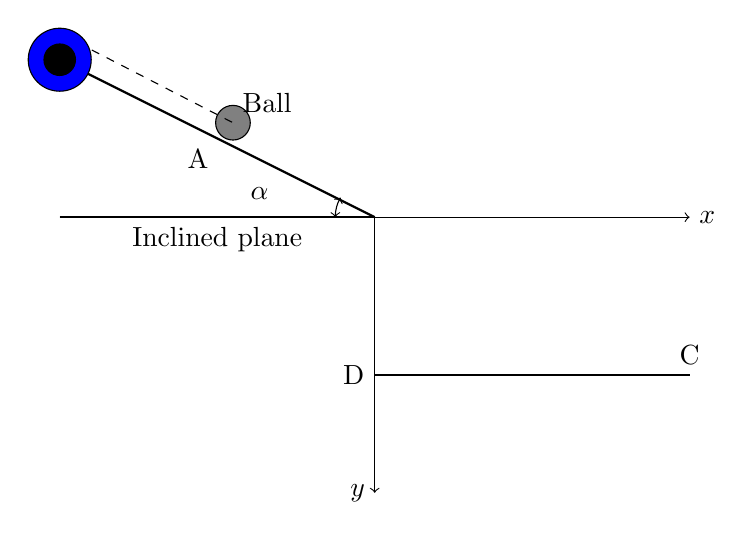
\begin{tikzpicture}
  % Inclined plane
  \draw[thick] (0,0) -- (4,0);
  \draw[thick] (4,0) -- (0,2); % Angle specified clockwise from the positive x-axis


    \draw[thick] (4,-2) node[left]{D} -- (8,-2) node[above]{C};
  
  % Disk
  \draw[fill=gray] (2.2,1.2) circle (0.22);
  
  % Line segment connecting the ball and the disk
  \draw[dashed] (0.22,2.22) -- (2.2,1.2);
  
  % Ball on the inclined plane
  \draw[fill=blue] (0,2) circle (0.4);
  \draw[fill=black] (0,2) circle (0.2);
  
  % Angle label
  \draw[<->] (3.5,0) arc (180:150:0.5);
  \node[right] at (2.3,0.3) {$\alpha$};
  
  % Lines representing x and y directions
  \draw[->] (4,0) -- (4,-3.5) node[left] {$y$};
  \draw[->] (0,0) -- (8,0) node[right] {$x$};
  % Labels and annotations
  \node[below] at (2,0) {Inclined plane};
  \node[above right] at (2.2,1.2) {Ball};
  \node[above right] at (1.5,0.5) {A};
\end{tikzpicture}

     \end{center} 
\begin{enumerate}

	\item On libère le corps S du point A sans vitesse initiale et il glisse sans frottement sur le plan incliné provoquant la rotation du
cylindre. 
    \begin{enumerate}
        \item Déterminer l'accélération du corps S et en déduire la nature de son mouvement.
        \item Déterminer la vitesse v1 du corps S au point O sachant que OA= 2m.
    \end{enumerate}
\item Au point O le fil se détache du cylindre à un instant t=0 et le corps S tombe au point C d'une altitude OD=75cm. 
    \begin{enumerate}
        \item Donner les équations horaires du mouvement du centre d'inertie du corps S dans le repère (O,x,y).
        \item En déduire la durée de chute du corps S. et La distance DC.
    \end{enumerate}
\item Lorsque le fil se détache du cylindre, ce dernier est soumis à un couple résistant de moment constant $M_{\Delta} = -7,5.10^{-2}N.m$,et il s'arrête de tourner après avoir effectué plusieurs tours. 
\begin{enumerate}
    \item Déterminer l'accélération angulaire $\ddot{\theta}$ du cylindre. 
	\item 3-2-Quel est le nombre de tours effectué par le cylindre durant le freinage.
\end{enumerate}
\end{enumerate}


   \end{Box2}


%%_________________________Exercice !2 :"_________________________Exercice
\begin{Box2}{Exercice 2 :une poulie à double gorge }
   % \begin{wrapfigure}[1]{r}{0.32\textwidth}
  %\begin{center}
	  %\vspace{-0.6cm}
	%\includegraphics[width=0.32\textwidth]{./ex_01.png}
  %\end{center}
%\end{wrapfigure}
  On considère une poulie à double gorge de rayons $R_1=10cm$ et $R_2=20cm$ qui peut tourner sans frottement autour d'un axe $\Delta$ fixe. Les deux corps $S_1$ et $S_2$ sont suspendus par deux fils inextensibles enroulés sur les poulies comme l'indique la figure.

\begin{center}
    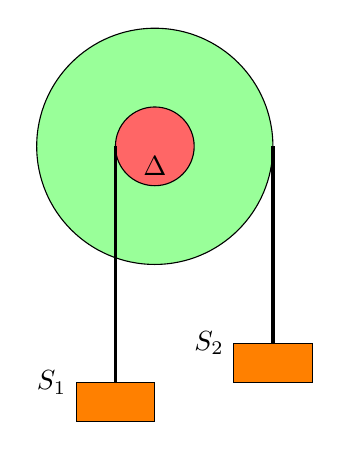
\begin{tikzpicture}
  % Draw the pulleys
      \draw[fill=green!40] (0,0) circle (1.5) ; % Pulley 2
      \draw[fill=red!60] (0,0) circle (0.5) node[below] {$\Delta$}; % Pulley 1
  
  % Draw the ropes
  \draw[very thick] (-0.5,0) -- (-0.5,-3); % Rope connected to pulley 1
  \draw[draw=black, fill=orange] (-1,-3) node[left] {$S_1$} rectangle ++(1,-0.5);

  % Draw the ropes
  \draw[very thick] (1.5,0) -- (1.5,-2.5); % Rope connected to pulley 1
  \draw[draw=black, fill=orange] (1,-2.5) node[left] {$S_2$} rectangle ++(1,-0.5);
  % Add labels
  %\node at (0,-1.5) {$P_1$};
  %\node at (0,-2.5) {$P_2$};
\end{tikzpicture}
\end{center}


\textbf{Données : }
\begin{itemize}
    \item Moment d'inertie de la poulie à double gorge : $J_{\Delta} = 2.10^{-2}kg.m^2$

\end{itemize}

\begin{enumerate}

	\item 	Déterminer l'expression de $m_2$ en fonction de $m_1$ , $R_1$ et $R_2$ pour que la poulie reste en équilibre.
    \item On utilise par la suite $m_1=1kg$ et $m_2=0,7kg$ puis on libère le système sans vitesse initiale à un instant t=0. 
		\begin{enumerate}

			\item Déterminer le sens du mouvement. et Montrer que l'accélération angulaire du système des deux poulies est:
                $$\ddot{\theta} = \frac{g(m_2.R_2 - m_1.R_1)}{m_1.{R_1}^2 + m_2.{R_2}^2 + J_{\Delta}}$$
                Calculer sa valeur.
            \item Quel est le nombre de tours effectués par le système des deux poulies {P1+P2} pendant la durée t=2s.
		\end{enumerate}

\end{enumerate}

\end{Box2}

\begin{Box2}{Exercice 3 : moment d’inertie }
  Un anneau de moment d’inertie $J_{\Delta}$ tourne autour de son axe ($\Delta$) avec 90 tr/min .
Pour freiner cet anneau , on exerce sur lui un couple de forces de moment constant
$M_c = -0,2N.m$. m jusqu’à son arrêt.
On néglige les frottements.
\begin{enumerate}
  \item Quelle est la nature du mouvement de l’anneau pendant l’application du couple
résistant ? Justifier la réponse  
\item Calculer la valeur de l’accélération angulaire $\theta$ de l’anneau pendant l’action du
  couple de freinage avec $J_{\Delta} = 8.10^{-3}kg.m^2$.
\item Calculer $\Delta{t}$ la durée de freinage.

\end{enumerate}
\end{Box2}
	%\vspace{-0.8cm}


\begin{Box2}{Exercice 4 :Les toboggans}

  \begin{wrapfigure}[8]{r}{0.24\textwidth}
  \vspace{-1cm}
%%\begin{wrapfigure}[3]{r}{0.33\textwidth}
  \begin{center}
    \includegraphics[width=0.24\textwidth]{./exercice44.png}
  \end{center}
\end{wrapfigure}
Un système (S) est constitué de deux cylindres homogènes (D) et (D’) de même substance , de même épaisseur, coaxiaux,
solidaires l’un de l’autre. Le moment d’inertie
de (S) par rapport à son axe de révolution
  est $J_{\Delta} $=$ 1,7.10^{-1}kg.m^2$.

On enroule sur chaque cylindre un fil inextensible de masse négligeable . Soit $f_1$ le fil

enroulé sur $D_1$ de rayon $r_1$ à son extrémité
on suspend un corps de masse $m_1 $=$ 3kg$
et soit $f_2$ le fil enroulé sur le cylindre

$D_2$ de rayon $r_2 = 2r_1 = 40cm$, à son extrémité on suspend un corps de masse $m_2 = 2kg$.
On libère le système sans vitesse initiale.


\begin{enumerate}
  \item Montrer que le système est en mouvement dans le sens indiqué sur la figure ci-contre.
  \item En réalisant une étude dynamique montrer que l’équation différentielle vérifiée par $\ddot{\theta} = \frac{d^2\theta}{dt^2}$, peut s’écrire sous la forme suivante : $$\ddot{\theta} = \frac{r_1.g(2.m_2 - m_1)}{J_{\Delta} + r_1^2.(4.m_2 + m_1)}$$
  \item En déduire les valeurs de l’accélération linéaire $a_1$ de corps de masse $m_1$ et $a_2$ de corps de masse $m_2$.
  \item Calculer les deux tensions $T_1$ de $f_1$ et $T_2$ de $f_2$.
  \item À l’instant t = 0 les deux corps se trouve de la même hauteur du plan horizontal
    (h=0.5m ) et que le centre d’inertie du corps $m_2$ soit confondu avec l’origine de l’axe
Oz qui est orienté vers le bas.

On considère le point M contact entre le fil $f_2$ et $D_2$ voir figure .Trouver les caractéristiques du vecteur accélération $\vec{a_G}$ en ce point M à un instant t où le corps $m_2$ descend de $h_2$.

\end{enumerate}

\end{Box2}




\begin{Box2}{Exercice 5 : Etude du mouvement du centre de gravité d’une balle. }
%%\begin{wrapfigure}[3]{r}{0.33\textwidth}
	%%\vspace{-0.8cm}

  On considère un disque, de masse $m = 200 g$ et de rayon $r = 5 cm$, susceptible de
tourner autour d’un axe ($\Delta$). On applique au disque immobile un couple de forces de
moment M constant, le disque effectue alors un mouvement de rotation autour de
l’axe ($\Delta$). Au bout d’une minute, la vitesse angulaire du disque a la valeur de $\dot{\theta} = 5 rad/s$, à cet instant on supprime l’action du couple de forces.

Les frottements sont supposés négligeables.

\begin{enumerate}
  \item Calculer la valeur du $J_{\Delta}$ moment d’inertie du disque par rapport à l’axe ($\Delta$).
  \item Montrer que l’accélération angulaire $\theta$ du disque est constante au cours de
l’application du couple de moteur. Calculer sa valeur.
\item En déduire la valeur du moment $M$ du couple moteur.
\item Quelle est la nature du mouvement du disque après avoir supprimé l’action du couple
moteur ? Justifier la réponse.

\end{enumerate}
\end{Box2}


%\begin{center}
   %\Large{ \em{Exercices Supplémentaires}}
%\end{center}

%\vspace{-0.8cm}

%%%_________________________Exercice ! 3:"_________________________Exercice
%\begin{Box2}{Exercice 6:Etude du mouvement d’une balle de golf dans le champ de pesanteur uniforme }
%%\begin{wrapfigure}{r}{0.4\textwidth}
 %%\end{wrapfigure}

%\end{Box2}

%%_________________________Exercice 4 : _________________________Exercice
%\begin{Box2}{Exercice 7 :Le ski }
   %% \begin{wrapfigure}[12]{r}{0.5\textwidth}

%%\end{wrapfigure}


%\end{Box2}
\begin{center} \emph{\textbf{“The physical universe and its buzzing machinery, its fantastical scenery.”}}
\end{center}

%\vspace{-0.6cm}
%%%_________________________Exercice 5 : _________________________Exercice
%\begin{Box2}{Exercice 4 : }
   %% \begin{wrapfigure}[14]{r}{0.5\textwidth}
  %%\begin{center}
	  %%\vspace{-0.6cm}
	%%\includegraphics[width=0.5\textwidth]{./img/ex5.png}
  %%\end{center}
%%\end{wrapfigure}

%4

%\end{Box2}

%\begin{Box2}{Exercice 5 : }

%44
%\end{Box2}


%\begin{Box2}{Exercice 6 : }


	%\end{Box2}


%\begin{Box2}{Exercice 7 : }
%\end{Box2}
\end{document}
